\documentclass[12pt]{article}
\usepackage[utf8]{inputenc}
\usepackage{amsmath, amssymb}
\usepackage{graphicx}
\usepackage{hyperref}
\usepackage{enumitem}
\usepackage{geometry}
\geometry{margin=1in}
\usepackage{biblatex} %Imports biblatex package
\addbibresource{bib1.bib} %Import the bibliography file


\title{CSC111 Project2}
\author{Jiyi Yang, Yifu Liang, Sida Luo, Kaiwen Yang}
\date{2025.Mar.30}

\begin{document}
	
	\maketitle
	
	\section*{Introduction}
	\subsection*{Motivation/background}
	Imagine that you have just ordered your lunch in a random building at a junction on campus, and the app says that the courier is 100 meters away from you, finishing orders also on the campus. But as you continue to refresh the app to see the progress of the delivery, you find that the courier is now going further and further away from you. After the courier finishes a delivery so far away from you, he finally starts your order. After waiting for the courier to come back to you, you can finally have your lunch. You would wish that when your courier is approaching you, he is actually approaching you instead of going down the street and turning back. This is not the best way to deliver food since the courier is so close to you, and stopping here would result in less waiting time for the customer.
	
	The optimization of delivery routes matters and should be cared about because if the app cannot provide reasonable routes, there would be too much waste of time for couriers and customers during each order, and the income of couriers and stores could be affected by providing a bad user experience, making the situation negative for all stakeholders.
	
	\subsection*{Goal of project}
	To reduce the unnecessary wasting of time and money, we choose to find a way to optimize the delivery route so that all deliveries would be completed in the shortest time, by finding optimal paths between buildings on this campus.
	
	\subsection*{The degree of exploration (similarity to defined project)}
	Our project would be focusing on finding an optimal path that involves chosen destinations on campus with the least possible amount of time, so that all destinations would be visited. Turning back is an allowed option because there are cases where this is better than going around a block without any destination. And the project would be using Flask\cite{noauthor_welcome_nodate} to build up the front end and use Folium to create the interactive map (an OpenStreetMap), then the required computations would be performed in the back end. Apart from that, the project would use Google Maps API\cite{noauthor_googlemapsgoogle-maps-services-python_2025} \cite{noauthor_distance_nodate} to obtain the dataset, and would have its python modules developed based on Greedy Neighbour and Dijkstra’s Algorithm.
	
	\section*{Dataset description}
	Our graph data is stored in JSON format in the working directory with the name graph\_output.json. Inside it all the data that we get through the API is stored, and the JSON data is imported as a graph through json\_to\_class.py.
	
	The source of the JSON data is very complex: our most primitive data comes from Wikipedia, a list of buildings on the St. George's campus of the University of Toronto\cite{noauthor_list_2024}. We copied these lists in a CSV and called the Google map API via generate\_graph\_json.py to get the coordinates of the buildings, distances to other buildings, and walking times, and connected the vertices that met the conditions according to the conditions we set in our Proposal as edges to form a graph.
	
	The difficulty with this python script for calling APIs is that if we just call the APIs sequentially, there are about 180 buildings in total that will call the API 180\textsuperscript{2} times, which not only increases the time it takes to fetch the data, but also gets charged a high fee for calling a large number of APIs. So we learned that Google Maps provides a Matrix API that can be used for us to call a matrix of results at once, but there is still a limit each time. Therefore, we optimized the algorithm for calling the API, which is represented as follows:
	\begin{figure}[h]
	    \centering
	    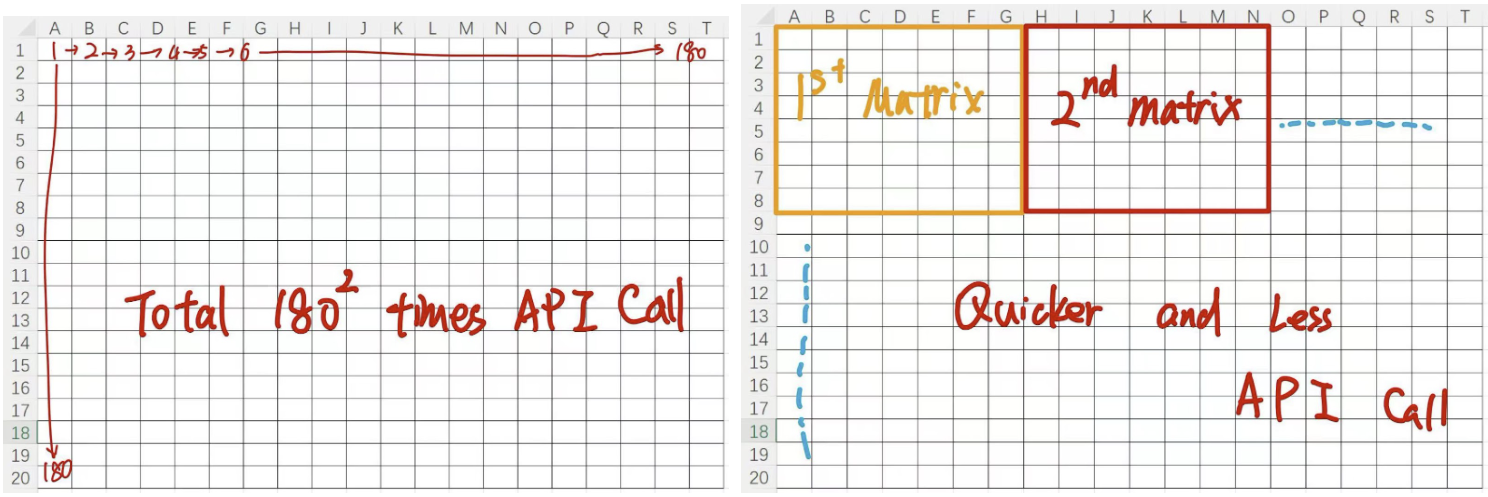
\includegraphics[width=0.9\linewidth]{image.png}
	    \label{Old VS New}
	\end{figure}
   
	
	\subsection*{Datasets import}
	The JSON file will initially be imported as a graph by json\_to\_class.py, and will also provide markers storing latitude and longitude information for all locations, which will be called by folium to display an interactive point on the map.
	This part of the project is rather routine and I did not encounter any very challenging situations.
	
	\section*{Computation overview}
	\subsection*{Design of graph/use of graph}
	\subsection*{Overall program structure}
	The whole program can be mainly divided into three parts:
	\begin{itemize}
		\item Methods related to loading .json into a Graph class instance
		\item Methods used to compute the shortest path to several destinations
		\item Methods used to generate the map and path according to the computation result
	\end{itemize}
	
	Methods related to load data (those in file json\_graph\_from\_json.py) are similar to methods that we do in ex3 and ex4. Firstly, it loads every node from the datasets, then another loop is used to load every neighbour for these nodes as edges of the graph. Since our datasets ensure every node is connected, there is no need for us to deal with situations where some nodes are isolated from the rest of them, leading some nodes to be unable to be reached from their unconnected nodes.
	
	Methods related to computation (in pj2\_graph.py and pj2\_graph.alg) are mainly designed based on Dijkstra’s Algorithm\cite{noauthor_dijkstras_2025}. The method input to get the smallest path between several nodes is the starting point name and a list of names of locations that are desired to be reached (whose first element of the list is the starting point). By inputting this informations, the method will generate a list that represents order of location user can traverse every destination from the starting in the shortest time. It is worth noting that the list may include some locations that are not in destinations, since the destinations may not be adjacent to each other, but be connected to some other nodes. These ‘undesirable’ locations are used to ensure users can move to destinations in a reachable path.
	
	Methods used to generate the map and path according to computational results are in the main module (main.py), the index() function utilizes Folium to generate the map and iterates through nodes loaded from a JSON file to generate markers. Each marker, representing a node, includes a clickable button that appends its label to the clickedMarkers list via the JavaScript function sendClickedNodes(), while the clearSelection() function is available to reset the selected markers. When markers are selected, their coordinates—stored in the global variable last\_path—are used by Folium’s polyline method to draw the route on the map. This dynamically generated map is then saved as an HTML file in the templates folder and rendered using Flask’s render\_template function. Meanwhile, the calculate() function (referred to as part of the overall routing logic) calls functions from the integrated graph modules to determine the optimal arrangement of nodes and compute the shortest path’s distance, thus combining back-end algorithmic processing with front-end interactive display.
	
	\subsection*{Computation method}
	The computation method we use to compute the fastest path is similar to the mindset of ‘Nearest Neighbour Method’\cite{noauthor_nearest_nodate} in Travelling salesman problem\cite{noauthor_travelling_nodate} (ie, TSP), but there are some differences. In the nearest neighbour method, we are asked to find a path that traverses every node in the graph and returns the starting node. However, in our topics, only several nodes are required to be reached, and there is no requirement to return to the beginning. Therefore, several changes are made.
	
	The main difference between our topics and TSP is that we don’t need to traverse every node in the graph, but only several nodes in it. For this reason, a method (generate\_complete\_graph, in pj2\_graph)  used to shorten the original big graph into a smaller graph is called to deal with it. By making the destinations the only nodes in the shortened graph, we can similarly design methods from our reference, decomposing our problem into smaller.
	
	However, it is worth noting that shortening the graph into a shorter one directly by reloading a graph only on destinations is incorrect, since some destinations are not adjacent, and directly loading may lead these nodes to be connected. Additionally, even if two nodes are adjacent, it is possible that there can be a path that is faster than the weight between these two nodes. To deal with this complicated situation, Dijkstra’s algorithm is introduced.
	
	To generate a reliable shortened graph, Dijkstra’s Algorithm, which can generate the shortest distance between two points, is introduced. The method ‘dijkstra’ is designed to return a dictionary that represents the distance and path between a node (start) and the rest of the nodes. Since we already know where we need to go, we can generate a dictionary of dictionaries based on our destinations, whose key is the node, and the value is the distance between this node to other nodes. After gaining this dictionary, we can generate a new graph that ensures the nodes are only destinations and adjacent to each other. And due to the use of Dijkstra’s algorithm, the weight of the edge must represent the shortest path, even if these two nodes are not adjacent in the original graph.
	
	After gaining a correct shortened graph, we need to consider the logic to determine the order of destinations to reach to guarantee the shortest path. In greed\_dijkstra (in pj2\_graph.py), we used a while loop to implement the logic of ‘always arriving at the nearest neighbour’. In each loop, we always go to the unvisited nearest neighbour by using the ‘get\_nearest\_path\_unvisited’ method in \_Vertex. After moving it to the nearest neighbour, it will be added to the visited (a set) to avoid repeating arrival. Then the nearest neighbour will be used as the new node in the next loop process. The loop will stop until every destination is reached, which means it is impossible to output a path that may not include every destination.
	
	\subsection*{Obtaining datasets and running of program}
	\begin{itemize}
		\item Library requirements for Flask. Folium.
		\item Download of datasets download the JSON file in the same folder as main.py.
		\item Running instructions: extract everything in a folder, create a folder called “templates”, run main.py, and click on the provided link in the console.
	\end{itemize}
	Changes from initial plan: restricted the area to the buildings involved in the St.George campus.
	
	\section*{Overall difficulty}
	Aside from the high level of difficulty of the code itself, the biggest challenge we faced was integrating the work of everyone on the team. Because each of us had a different understanding of the algorithm and, therefore, different requirements for what needed to be passed in and out, it led to a lot of bugs when we put together everyone's work, and we spent a lot of time trying to locate the problem and work out the bugs. This was especially true when the final presentation was incorrect and did not report an error, which could mean more than just a bug in an individual method. It could even be an error triggered by a chain of problems.
	So we learned a lot of teamwork skills in this project, how to communicate and design interfaces that can be widely accepted in the future. More importantly, we gained experience in using git.
	
	\section*{Discussion}
	\subsection*{Effectiveness}
	The project is highly effective compared to a brute-force enumeration method, as it leverages optimized graph algorithms like the greedy Dijkstra method to quickly approximate an optimal route without having to exhaustively search all possible combinations. This efficiency translates to faster computations and improved scalability when dealing with larger datasets, while the seamless integration of Flask and Folium creates an interactive and intuitive user experience. Users can dynamically select markers on an interactive map centered around the University of Toronto and immediately visualize the calculated route, which highlights the project’s practical utility in real-world applications.
	
	\subsection*{Proof of correctness}
	Let T be the list of k target nodes (with start $\in$ T).
	
	\textbf{Base Case (k = 1)}\\
	The set of targets is \{start\}.
	\\greedy\_dijkstra(start, [start]) initializes path = [start], and since all targets are already visited, it returns immediately.\\
	Correct, since the only required node is start.
	
	\textbf{Inductive Hypothesis}\\
	Assume that for any set of m target vertices (m $\geq$ 1), greedy\_dijkstra correctly constructs a path visiting all targets by repeatedly appending Dijkstra paths to the nearest unvisited target from the current node.\\
	That is, the result visits all m targets and respects Dijkstra's shortest path between each consecutive visited node.
	
	\textbf{Inductive Step: Prove for (m + 1) targets}\\
	Let the current set of visited targets be of size m, and we are now choosing the (m + 1)th target.\\
	The function runs Dijkstra from the current node and selects the nearest unvisited target $t_{min}$ based on the correct Dijkstra paths (by assumption).\\
	Since Dijkstra returns shortest paths, and we choose the minimum-cost one, the path from the current node to $t_{min}$ is shortest.\\
	The algorithm appends that path and adds $t_{min}$ to visited, growing the solution.\\
	By the hypothesis, all previous m targets were correctly added via shortest paths, and now the next one is added similarly.\\
	Thus, by induction, after visiting all targets this way, the full path consists of a valid traversal visiting all target nodes, using shortest paths between each consecutive pair.
	
	\subsection*{Limitation}
	For some typical cases, the Greedy Neighbour Algorithm wouldn’t give the very best route as the chosen node could be visited without getting some of the neighbours, in which the path would be better if this algorithm is not used. For example, two nodes on different sides of the Queen’s Park can be visited simply by going across the park, but the algorithm would give a path going around it because these two nodes are not neighbours.
	
	Additionally, the current system is built around static data loaded from a JSON file, which means that it cannot dynamically adjust to real-time changes such as traffic or weather conditions without significant modifications. The integration of Flask and Folium, while excellent for interactive visualization, may also pose challenges in scalability and responsiveness when faced with very large datasets or high-frequency user interactions.
	
	Moreover, once the map is rendered, the visualization remains static, requiring a complete re-render for any updates, which could limit its effectiveness in rapidly changing environments.
	
	\subsection*{Further exploration}
	A possible further exploration is to integrate real-time data sources, such as live traffic, weather conditions, and user feedback, into the current routing algorithm, thereby enabling dynamic route adjustments and predictive modeling. This enhancement could leverage advanced machine learning techniques to forecast congestion or delays and further refine the optimal path calculation. By building on the project's existing efficient graph-based method, which already outperforms brute-force enumeration, this extension would provide even more accurate and responsive route suggestions, ultimately elevating the user experience in complex urban environments while maintaining the system's high performance and scalability.
	
	
	\printbibliography
	
\end{document}